% ----------------------------------------------------------------------------------------
% This contains all the content under Part: Networking
% ----------------------------------------------------------------------------------------
\part{Networking}
\chapter{Basics}
Networking is all about enabling different devices to talk to one other. Here the term ``device'' may refer to computers or any other electronic entity. Thus the Internet connects many devices with one other and, in this case, the devices are computers. But when a computer is connected to many different USB devices via a USB hub, that is also networking. The network could be inside an IC where a CPU and a DMA Engine may be connected to a RAM, ROM and many hardware modules. This is also networking - In this case, the CPU, DMA, Memory Controller (RAM/ROM) are all ``devices''. \footnote{Though, traditionally the word ``networking'' is used to refer to computer networking like the Internet, this distinction is unnecessary - It is like calling linear algebra as ``signal processing''. When we do that, we unnecessarily confuse people into thinking it is a separate field and prevent them from applying techniques learned from Signal Processing on to solving non signal processing problems. In fact, concepts in Networking can be applied to not just electronic entities, but also to mechanical entities, like conveyor belts, road and train networks etc.}

Scenarios where devices talk to one another can be compared to scenarios where people talk to each other. For instance, take the scenario where a teacher is talking to a class. Most of the time, she is talking and all the students in the class are listening. This is a broadcasting scenario. But when a student has a question, he raises his hand - this conveys to the teacher that someone wants to talk and hence the teacher stops talking to let the student talk. Similary scenario may exists in a network, in which case, solutions applied for the human communications problem can be replicated for the devices: Notice that in the human communication problem, we avoid simultaneous talking of people, by using a visual way of communicating that the student wants to talk. Here one can think of two separate ``channels'' existing: One is the audio channel in which any one person can send information at a given time and a visual channel which is used to figure out who gets to occupy the audio channl. In terms of devices, we could similarly solve using two channels: The visual channel could simply be an interrupt line, where as the audio channel will be the actual data line(s). 

\section{CSMA/CD}
Imagine a bunch of individuals in a room. Say 10 people in the room want to have one-to-one conversation with ten others. To avoid chaos we allow only one conversation to happen at a give time. There are many ways to solve this problem. One is to use some sort of a round robin method: Every person in the room has a no. and there is a digital screen that basically changes number every 20 seconds. Only the person with the no. currently displayed on the screen is allowed to talk. This is a simple solution, but has a fundamental problem: Even if the person whose no. is currently displayed has nothing to say, still the next person in line has to wait for 20 seconds. This is such a waste of time. In such real world situations, normally what people do, is that they see if anyone is talking and when no one is, they start speaking. But if, just as they start talking, if someone else also starts talking, they will stop and let the other person talk. It is possible that, when two people start talking simultaneously, both may back off out of courtesy. And again one of them will try to start talking. Both may again start talking simultaneously....this can happen a bunch of times. And eventually one just stays silent for a longer time hinting that the other person may now talk.

What was described in the above paragraph is called \emph{Carrier Sense Multiple Access with Collision Detection} or \emph{CSMA/CD}. The very first wireline networks (and wireless networks even today) followed this. In this case, simply, a bunch of devices will all be connected to the same bus (a bunch of logically related wires) as shown below. When a device in this simple network wants to send data to another device, it will,
	\begin{enumerate}
	\item First observe, for an amount of time, if there is any activity happening on the bus
		\begin {itemize}
		\item If there is some activity going on, wait until the bus falls silent
		\item If or when the bus is silent, it can start sending data
		\end{itemize}
	\item Send data for a small quantum of time and simultaneously read back the data from the bus. Match the sent data with the read-back data
		\begin{itemize}
		\item If they don't match, then it means someone else also tried to talk during that past quanta and there was a data clash. Stop sending data and go back to step 1
		\item In they do match, continue sending data
		\end{itemize}
	\end{enumerate}
	
To avoid any one device hogging the bus for a long time, we can set a rule that no one can keep talking beyond a stipulated period of time.

\section{Network Switch}
In modern wireline networks, single bus based networking is rarely found. Instead some sort of a switch is employed as shown below. The switch typically contains on dedicated bus between each pair of devices that would ever want to talk to each other - for now, let us assume that every device would like to, at some point, talk to every other device on the network. Now, if a device, say device A, wants to talk to device B, it will simply raise a flag and the switch, if no one else is talking to device B, will ``enable'' the connection between A and B and the communication will start. If two devices want to talk to device B at the same time, the switch will allow the higher priority device to talk first. If both devices have the same priority, the switch will randomly allow one device (coin toss). Since the switch has a dedicated path for each device pair, the arbitration mentioned above is required only when two devices want to talk simultaneously to the same third device. But if the two devices want to talk to two other devices, no arbitration is required. So while a A->B, C->B communication cannot happen simultaneously, a A->B, C->D can.

\section{Master and Slaves}
The idea of masters and slaves in a network is that, while master may initiate conversations, slaves will either only listen or reply when asked by a master - \emph{i.e.}, A slave will never initiate a conversation. In computer networks, one's laptop would be a master while a web server could be a slave. In ICs, typically CPUs, DMA engines etc., will be masters, while Memory Controllers, I/O Controllers will be slaves.

While a slave will never initiate a conversation, it may want to talk to a master. In this case, just like the teacher in a class room example, side channels are used to inform the master of the slaves ``wish''. The side channel may be elaborate or could be a single wire interrupt. And just as the teacher may either immediately pause and ask the student to go ahead, or wait for a while and then let the student talk (or completely ignore him), the master device may immediately enquire the slave or may wait for a while and then enquire or completely ignore it.Thus while the slave, may in an indirect way, want to talk to the master, granting that wish is up to the master. 


\chapter{OSI Model}
The most popular model used for networking computers, for long, has been the OSI model. It envisions networking using 7 layers of abstraction as shown in the diagram below (Courtesy: Wikipedia, ``OSI Layers'').

	\begin{table}[h] 
	\centerfloat
	\arrStr{1.3}	
	\begin{tabular}{l l p{0.5\textwidth} p{0.4\textwidth}}
	\toprule
	Layer & Data Unit & Function & Examples \\
	\midrule
	7. Application & Data & {\footnotesize High-level APIs, including resource sharing, remote file access, directory services and virtual terminals} & Mail, Internet Explorer, Firefox, Google Chrome \\
	6. Presentation & Data & {\footnotesize Translation of data between a networking service and an application; including character encoding, data compression and encryption/decryption} & ASCII, EBCDIC, JPEG\\
	5. Session & Data & {\footnotesize Managing communication sessions, i.e. continuous exchange of information in the form of multiple back-and-forth transmissions between two nodes} & RPC, PAP, HTTP, FTP, SMTP, Secure Shell\\
	4. Transport & Segments & {\footnotesize Reliable transmission of data segments between points on a network, including segmentation, acknowledgment and multiplexing} & TCP, UDP\\
	3. Network & Packet/Datagram & {\footnotesize Structuring and managing a multi-node network, including addressing, routing and traffic control} & IPv4, IPv6, ARP, IPsec, AppleTalk, ICMP\\
	2. Data Link & Bit/Frame & {\footnotesize Reliable transmission of data frames between two nodes connected by a physical layer} & PPP, IEEE 802.2, L2TP\\
	1. Physical & Bit & {\footnotesize Transmission and reception of raw bit streams over a physical medium} & DSL, Ethernet, USB\\
		
	\bottomrule
	\end{tabular}
	\caption{OSI Layers}
	\end{table}

The Physical layer is all about converting bits to signals that can be transmitted over a long distance and recovered back to bits. Hence it is a topic of digital communications that we will not deal with here. The top 3 layers are too high level and have such a wide scope that we cannot cover them here. So we will focus on the remaining 3 layers: Transport, Network and Data Link layers. We will occasionally say a thing or two about the rest.

Perhaps the best way of introducing networking is to talk about how data transaction and routing happens at every OSI layer. Since networking devices come at different levels of complexity, with each dealing with data transmission and routing up to certain layer in the OSI and being agnostic about layers above that. In fact, if we try to understand how various networking devices work, starting from the simplest and building up to more complex ones, we could get to grips with the basics of networking.

A \emph{Hub} is a ``Layer 1 device'' that understands only physical layer. Consequently it is the simplest of all networking devices. A Hub is simply a broadcaster/repeater. It has several ports. However, since physical layer is all about sending bits from one end to another, there is no concept of routing data. Hence a Hub broadcasts the bits it receives from any of its port to all other ports. Connecting many nodes to a Hub is the simplest approach to networking - we will simply be enabling a node to talk to more than one other node, with nodes ignoring data the Hub broadcasts to them, if it wasn't meant for them (This happens at the Data Link Layer level).  Without a Hub, a network can have a maximum of only two nodes! - one node directly connected to another. 

Hub are outdated. Originally they were cheaper compared to more complex network devices and could ``get the job done'', they are obviously pretty wasteful since they broadcast all the time. 

A \emph{Switch} is a ``Layer 2 device'' that understands up to Data Link Layer level. A Swich routes data from one of its ports to another using a Data Link Layer address called \emph{MAC address}. When several nodes are connected to a Switch for the first time, the Switch doesn't know the MAC address any of the nodes. Consequently, for some time, it behaves like a Hub - When a Switch receives a Data Link Layer frame on one of its ports, say, port 1, for the first time, it looks into the frame header and notes down the source MAC address found in it against the port 1. But, since it has no idea which of its ports is connected to the node indicated by the destination MAC address in the frame, it simply broadcasts the frame to all other ports. The nodes that receive this frame, examine if the frame belongs to them by matching the destination MAC address in the frame to their own MAC address. Only the actual destination node then responds to the source with a frame while other nodes simply ignore it. So on the way back, when the Switch grabs this return frame, and note down the sender's MAC address against the port it received it in - say, port 2.  Thus it slowly gains knowledge of the which of its ports is connected to which MAC address. So after a while, there won't be any unnecessary broadcasting.

A \emph{Router} is a ``Layer 3 device'' that understands up to the Networking layer. We will see how a router works in a while. But first, let us understand more about the Networking layer. As it's name implies, this is the layer primarily responsible for networking. This layer uses an addressing scheme called the IP address. Even though it may appear like MAC address is used to connect several nodes and nodes communicated with each other using MAC addresses, it is not true. When a node, say, node A, wants to talk to another node, say, node B, it doesn't right away start sending frames with node B's MAC address. Node A initially knows only node B's IP address \footnote{Either we manually enter node B's IP address into node A's application or DNS may be used. We will talk about this in the next section}. It needs to find out the MAC address of node B in order to start communicating with it - This is because MAC address is the lowest level of address in a network and without it data cannot be moved around in a network\footnote{For instance, if there is a switch in the network, it cannot understand IP addresses, but only MAC addresses}. To find out node B's MAC address, node A uses a network layer protocol called \emph{Address Resolution Protocol}  or \emph{ARP}. Basically, node A sends puts an ARP message on the network which tells a switch to intentionally broadcast to all the nodes connected to it. All the nodes receive the ARP message and the node that sees the destination IP address match with its own will reply, while others ignore. In the reply, node B will stamp its MAC address in the message and send it to node A's. Node A will thus build a table over time with IP addresses of nodes against their MAC addresses. Note that when node B receives the ARP from node A, it would have made a note of Node A's MAC address before sending the reply.

\section{Connecting Two Local Networks}
In the above paragraphs, notice how we didn't need a router for two nodes to talk to each other? Well, we don't need a router as long as the nodes in a network want to talk only to other nodes in the same network. So, what do we mean by ``same network'' here? How do we say that two nodes are on the same network and not on different networks? In fact, what does a ``different network'' mean? To answer these questions, imagine two networks shown below. Each consist of a bunch of nodes connected to each other using a hub.

	\begin{figure}[h]
	\centering
	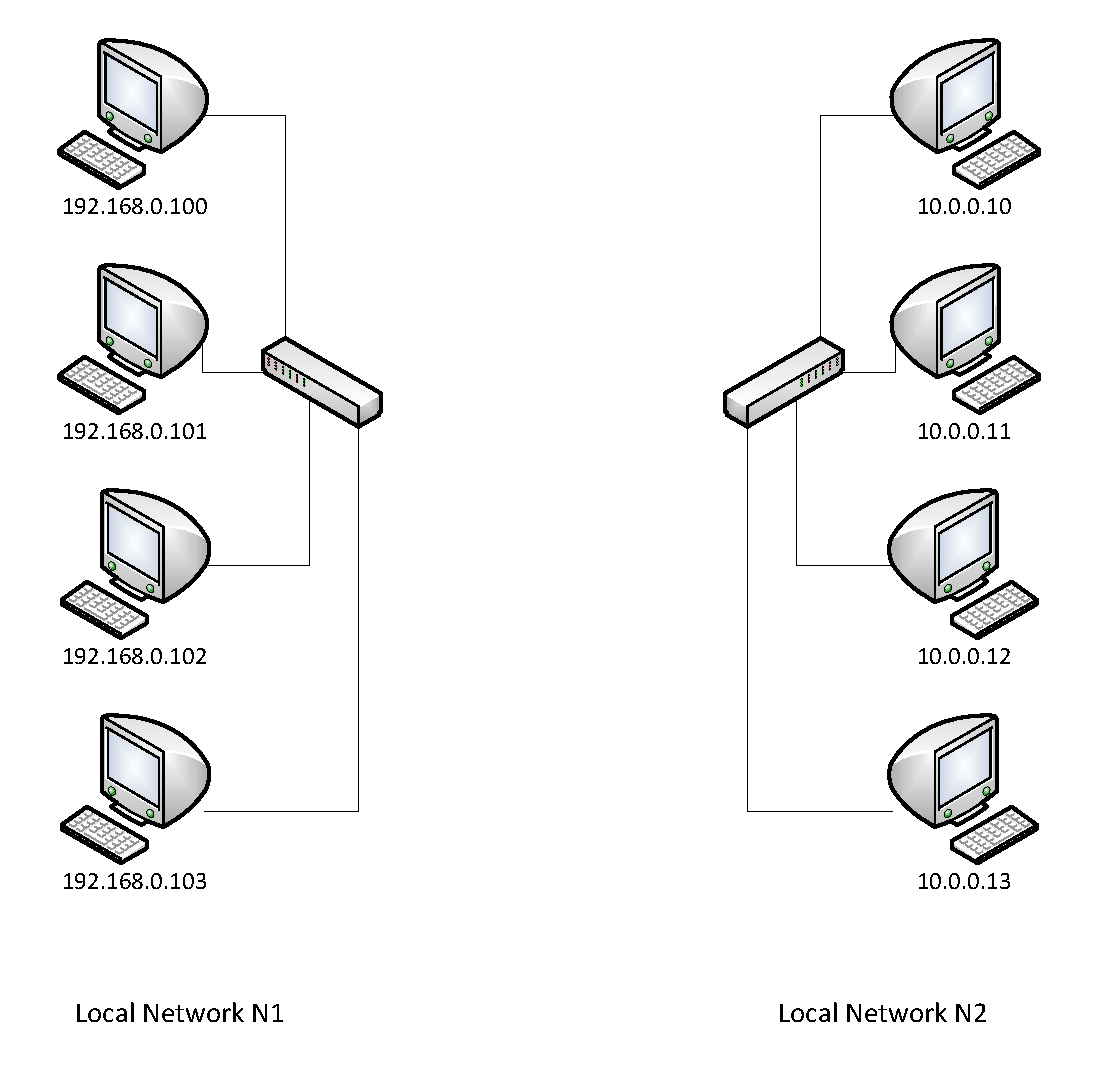
\includegraphics[width = \textwidth]{partNW/TwoLocalNetworks}
	\caption{Two Local Networks}
	\label{fig:localNWs}
	\end{figure}

We know from the paragraphs preceding this section how nodes in each network will talk to another node in its network - we will call this its ``local network'' from here on. We know how each node will build a table of IP addresses against MAC addresses of other nodes in its local network and how the hub builds a table of MAC addresses against its ports. But what if a node in the network N1 wants to talk to a node in network N2? For that we need routers. Routers are essentially what define a local network. The following figure depicts this. 

	\begin{figure}[h]
	\centering
	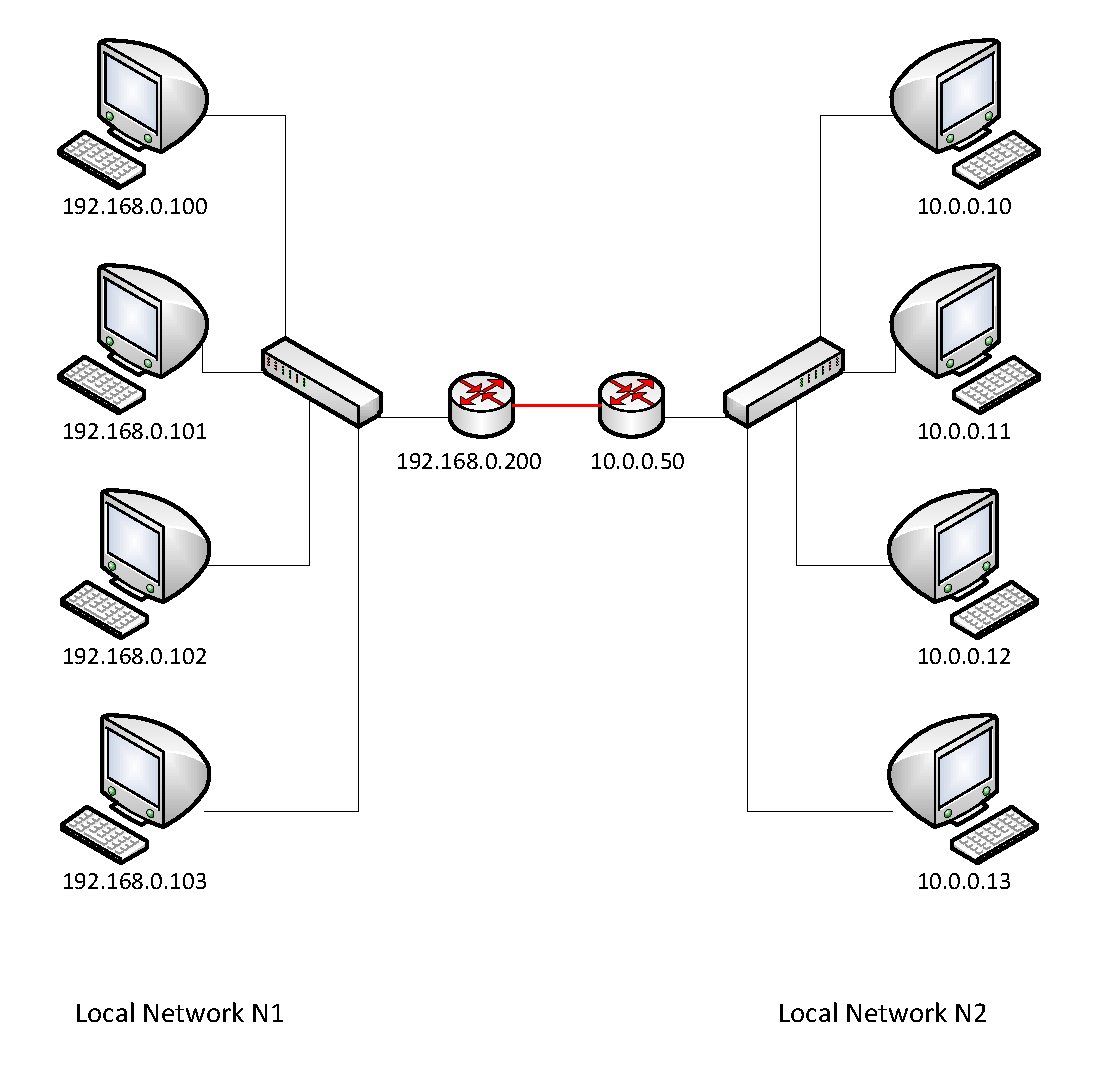
\includegraphics[width = \textwidth]{partNW/RouterConnectingNetworks}
	\caption{Inter Network}
	\label{fig:routerConnectingNWs}
	\end{figure}

The way it works is that, the user of a node, say 192.168.0.100, in network N1 would enter the network properties in the node as shown below. 

	\begin{figure}[h]
	\centering
	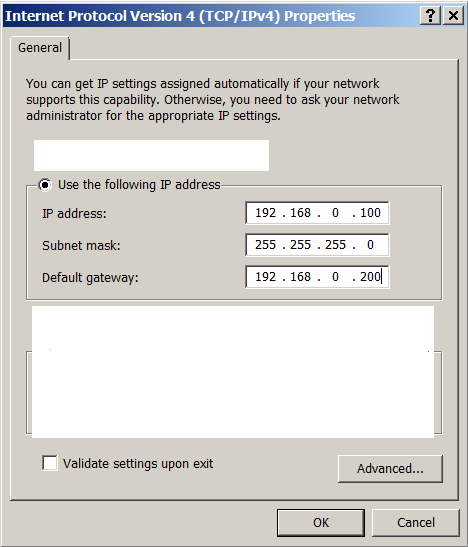
\includegraphics[width = 0.75\textwidth]{partNW/IP4Properties}
	\caption{Network Properties}
	\label{fig:ipv4DialogBox}
	\end{figure}

When this node wants to talk to another node in N1, say 192.168.0.102, the node applies the \emph{Subnet Mask} on this IP address (logical AND) and sees if the result matches 192.168.0.0. In our case, it does, and this means this IP address is in the same network, i.e., N1. At this point, the node 192.168.0.100 proceeds to find out the MAC address of the destination node, 192.168.0.102 (if it already doesn't know), using ARP, so that it can start talking to it. And we know how the rest will work.

Now consider the case when the source node, 192.168.0.100 wants to talk to 10.0.0.10. Again, it applies the subnet mask, but the result, 10.0.0.0 doesn't match its N1's 192.168.0.0. The source node thus understands that the destination node is not in its own network, i.e., N1. In this case, the source node doesn't try to find the destinations MAC address. Instead it simply stamps the message with the router's MAC address and sends the message to the router. Note that the message will still have the destination IP address of 10.0.0.10 - only the MAC address will be that of the router's. How does the source node know the router's IP address? It is because the user enters it in the ``Default Gateway'' field of the network properties dialog box\footnote{Note that, if the source node doesn't know the router's MAC address, it will again have to first use ARP to find that out}. The router looks at the message it received from the source node, examines the destination address and realizes that it doesn't match with its own IP address - it means the message was actually meant for someone outside network N1. So the message is sent to the router on N2\footnote{In our simple case, router on N1 is connected only to the router on N2 and no other router. So whenever it receives a message meant for a node outside its network, it has no other choice but to send to N2. We will talk later about what happens in the case of the router on N1 connected to many other routers - how it will know the destination node is in N2}. This is accomplished by the router on N1 changing the destination MAC address of the message (from its own MAC address) to match the MAC address of the router in N2. Again, only the destination MAC address is changed, but the IP address is left intact as 10.0.0.10. Router on N2 receives the message, and just like the router on N1, realizes that the message isn't meant for it. However, it understands that the destination IP address is in its own network and forwards the message to the switch in N2 which then sends the message to the destination node. 

\subsection{The Internet}
The internet is nothing but a lot of local networks connected together using routers. We just saw how nodes from two local networks can talk to each other with the help of routers. In this case, the routers, which were the ``gateways'' of these local networks were directly connected to each other. This is an oversimplistic possibility, one which will be impractical to use while connected so many local networks together to form the internet - obviously every local networks gateway cannot be connected to all other gateways. It is actually not required that the gateways of two local networks be directly connected to each other to enable communication between them. In fact, the essence of routers comes clear only when the local networks are \emph{not} connected directly to each other. The figure below shows how two local networks will actually be connected on the internet.

	\begin{figure}[h]
	\centerfloat
	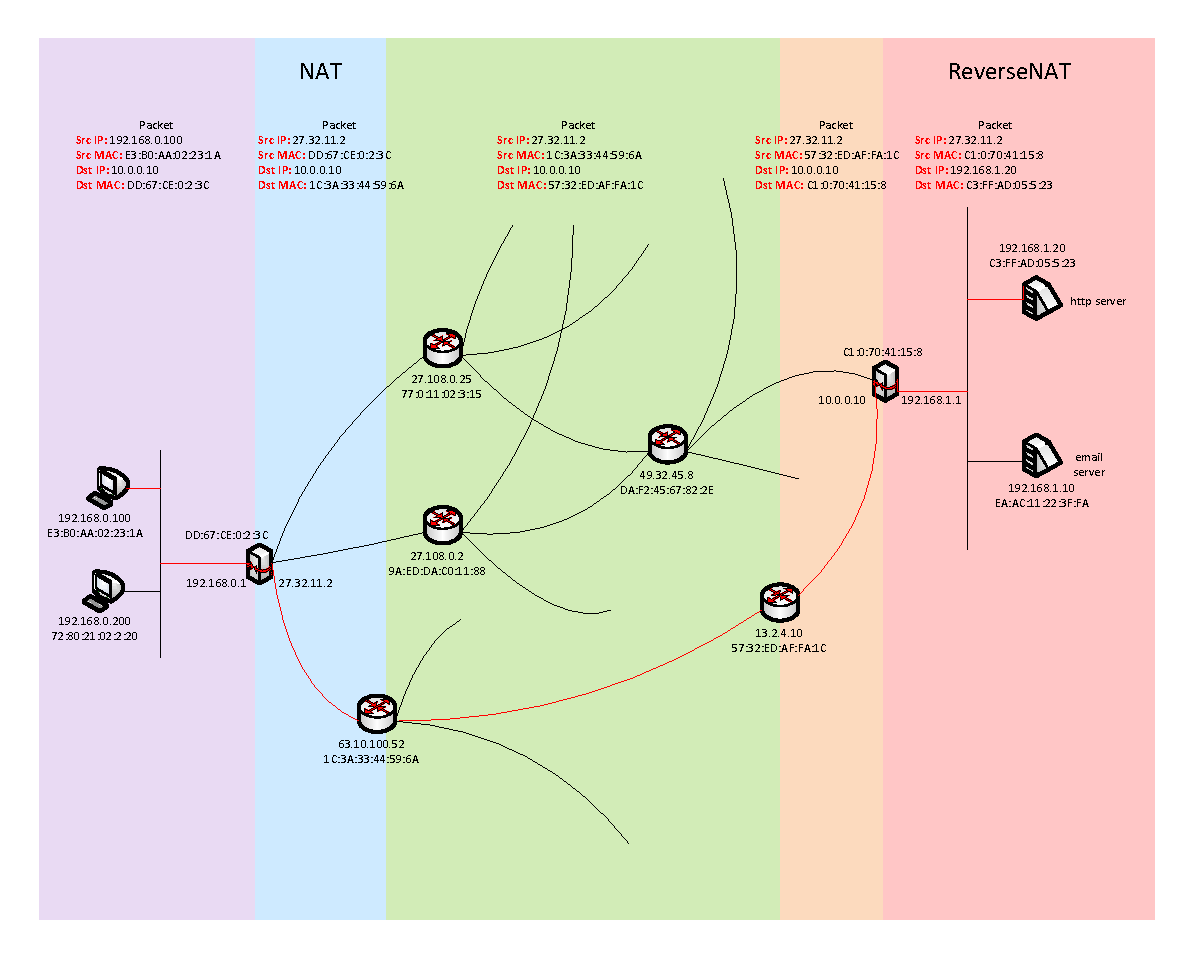
\includegraphics{partNW/internet}
	\caption{The Internet}
	\label{fig:internet}
	\end{figure}

Compare this with the simplistic version where gateways were directly connected to each other. The difference is that, in the simplistic version when the gateway of N1 realized that the packet sent by 192.168.0.100 wasn't meant for it, as the destination IP address, 10.0.0.10 doesn't match its own IP address, and forwards the packet directly N2. But in the real world, the gateway now has to send it to one of the routers R1, R2, R3. But which one of these will it choose? The answer is a little complicated, and we will deal with it later, but for now, let us just say that every router keeps a table that indicates which one of the routers it is connected to lies on the shortest path to the destination IP address. This is called the \emph{routing table}. The data in the routing table a best estimate and the router doesn't know whether it is a fact. Actually the routing table data keeps changing from time to time - This is where the whole idea of routing and that of the internet itself becomes interesting: This means that, the gateway of N1, which is also a router, may not choose the same router, that it chose to send the first packet to 10.0.0.10, for the following packets as well. In our case, we show that it chose R3 because its routing table said that R3 was on the shortest path to 10.0.0.10. But, suppose, after sending this packet, its routing table changed,\footnote{We will see later how routing table is built and how it evolves} now it may think R1 is on the shortest path to 10.0.0.10 and send the next packet to R1. The same logic applies to how the first level routers R1, R2, R3 will then forward the packet. In other words, every \emph{IP Packet} can potentially follow completely different routes from the source to the destination. This idea is called \emph{packet switching} and this is the genius of the internet. 

\subsubsection{Network Address Translation}
While discussing interconnecting two local networks, it was mentioned that the gateway of N1 changes the source MAC address of the data sent out to its own but leaves the source IP address intact. This is true only if \emph{Network Address Translation}(NAT) is not turned on in the gateway. In the case of internet and most networks, NAT is almost always enabled for all gateways. NAT is all about translating all the IP addresses in a local network to a 




